\documentclass[a4paper, 12pt]{article}


\usepackage[french]{babel}
\usepackage[utf8]{inputenc}
\usepackage[T1]{fontenc}
\usepackage{lmodern}
\usepackage{listings}
\usepackage{graphicx}
\usepackage{amsmath}
\usepackage{amsfonts}
\usepackage{amssymb}
\usepackage{caption}
\usepackage{subcaption}
\usepackage[usenames,dvipsnames]{xcolor}


\setcounter{secnumdepth}{4}
% TAILLE DES PAGES (A4 serré)

\setlength{\parindent}{0pt}
\setlength{\parskip}{1ex}
\setlength{\textwidth}{17cm}
\setlength{\textheight}{24cm}
\setlength{\oddsidemargin}{-.7cm}
\setlength{\evensidemargin}{-.7cm}
\setlength{\topmargin}{-.5in}

% Commandes de mise en page
\newcommand{\fichier}[1]{\emph{#1}}
\newcommand{\nom}[1]{\emph{#1}}
\newcommand{\Fig}[1]{Fig \ref{#1} p. \pageref{#1}}
\newcommand{\itemi}{\item[$\bullet$]}

% Commandes de maths
\newcommand{\fonction}[3]{#1 : #2 \to #3}
\newcommand{\intr}[2]{\left[ #1 ; #2 \right]}
\newcommand{\intn}[2]{\left[\![ #1 ; #2 \right]\!]}
\newcommand{\intro}[2]{\left] #1 ; #2 \right[}
\newcommand{\intrsod}[2]{\left[ #1 ; #2 \right[}
\newcommand{\ps}[2]{\langle #1, #2 \rangle}
\newcommand{\mdelta}[1]{\boldsymbol{\delta_{#1}}}
%% \newcommand{\mdelta}[1]{\delta_{\textbf{#1}}}

\pagenumbering{arabic}
\graphicspath{{images/}}

\title{ASM-TP2 : ACP-régression en génétique} 
\author{Pierre Petitbon \and Florian Privé \and Xinrui Xu}
\date{}

\begin{document}

\maketitle

\section{Préparation des données}

\begin{enumerate}
\setlength{\itemsep}{20pt}

\item[1.a)] 
	OK

\item[1.b)]
Le script place toutes les origines des individus des données sur une carte du continent américain, suivant la latitude et la longitude. La carte obtenue correspond bien à celle du sujet. 

\begin{figure}[!h]
\begin{center}
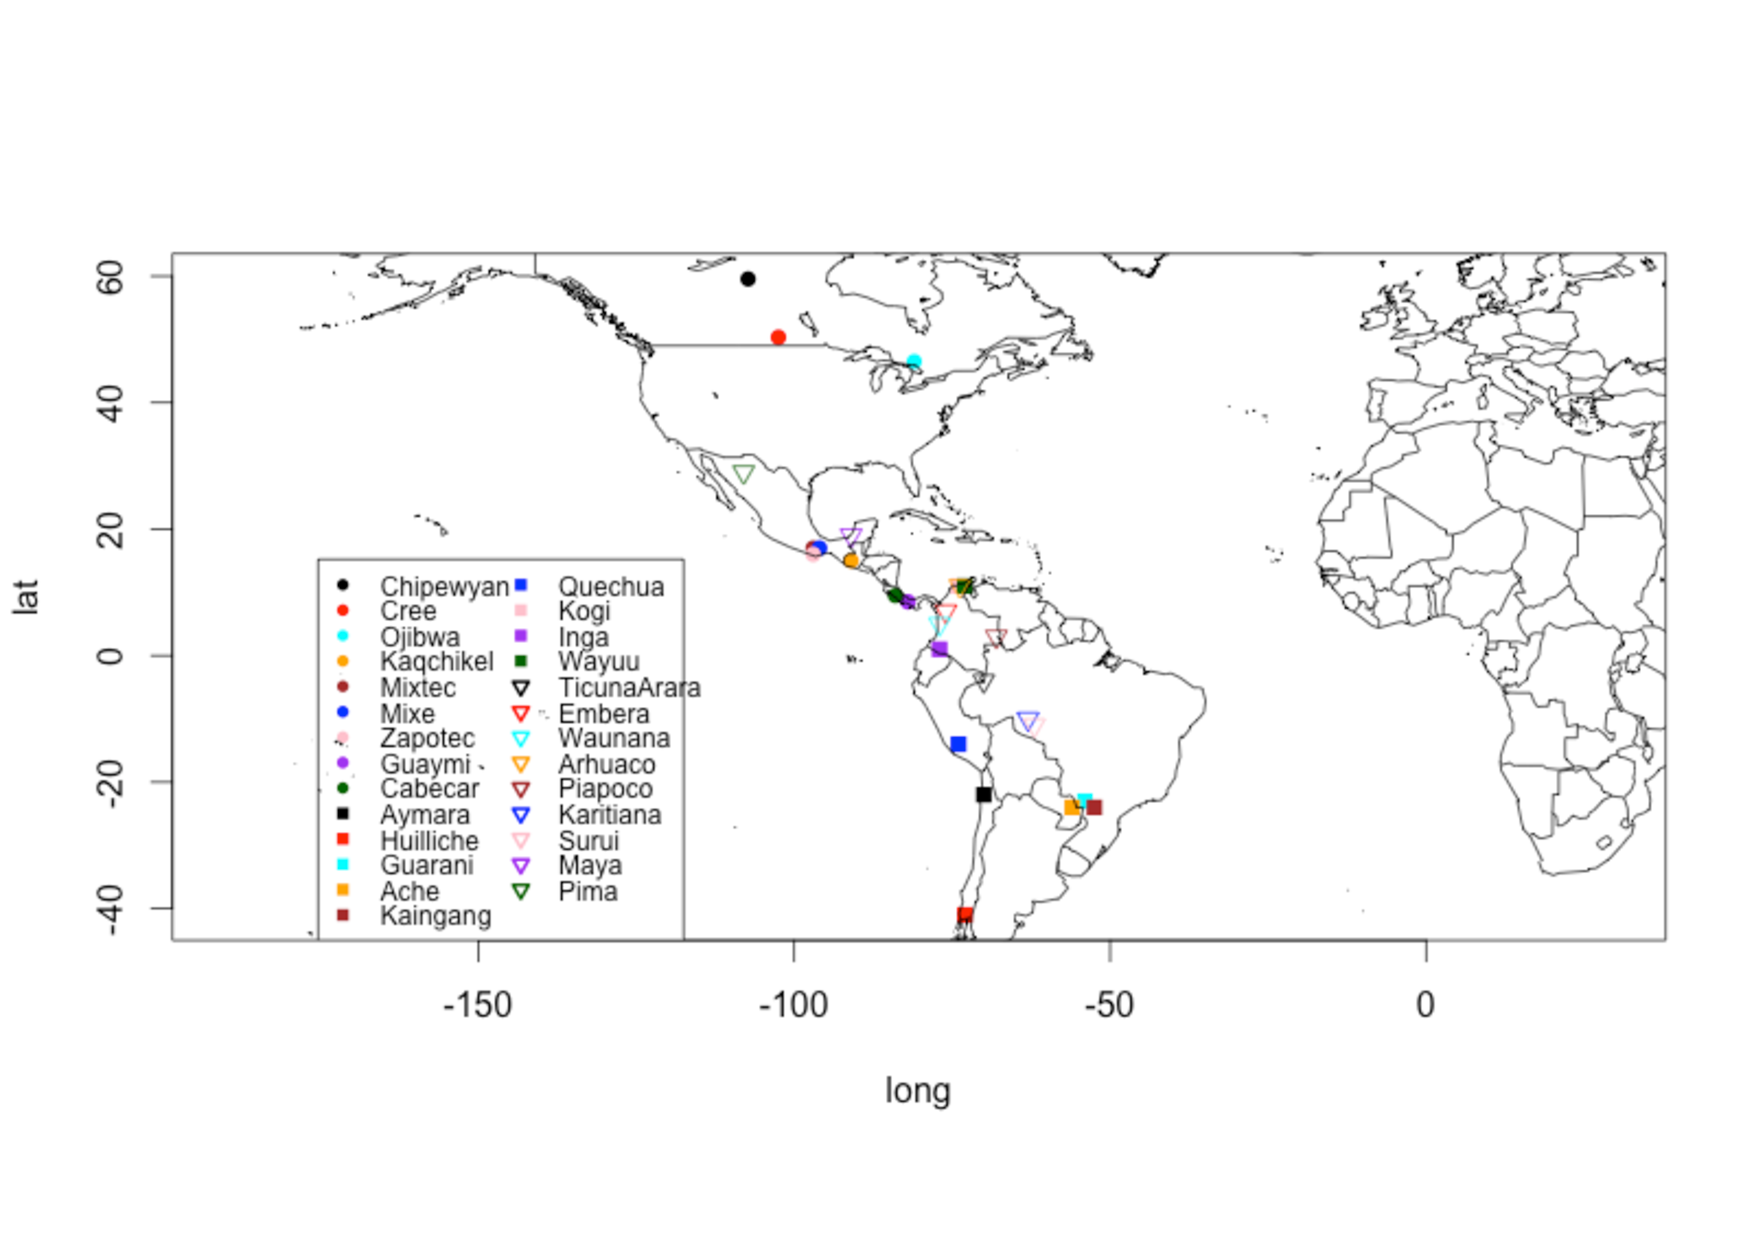
\includegraphics[scale=0.5]{Plot1b.pdf}
\caption{Répartitions des populations}
\end{center}
\end{figure}

\end{enumerate}


\section{Régression}
Le problème c'est qu'on est incapable de trouver les coefficients de la régression de la longitude car le nombre de marqueurs génétiques (5709) est beaucoup plus grand que le nombre d'individus (494). C'est pourquoi on régressera la latitude et la longitude avec les scores de l'ACP faite les marqueurs génétiques. 

À refaire (avec le cours) avec une démonstration mathématique.

\section{ACP}
\begin{enumerate}
\setlength{\itemsep}{20pt}
\item[3.a)]
 L'analyse en composantes principales consiste à transformer des variables corrélées en nouvelles variables décorrélées les unes des autres. Ces nouvelles variables sont appelées composantes principales. Elle permet de faire une analyse sur moins de variables et réduit la redondance de l'information. En pratique, elle projète des données un numbre réduit d'axes orthogonaux, tout en maximisant la variance des données projetées sur chacun des axes.

 \item[3.b)]
 On réalise une ACP sur les données génétiques avec tous les individus. 
 On n'a pas besoin d'utiliser l'argument scale car les variables (les marqueurs génétiques) n'ont pas d'unités de mesures : les valeurs sont binaires. Il n'y a donc pas besoin de mettre ces variables sur une même échelle. 

\begin{figure}[!h]
\begin{center}
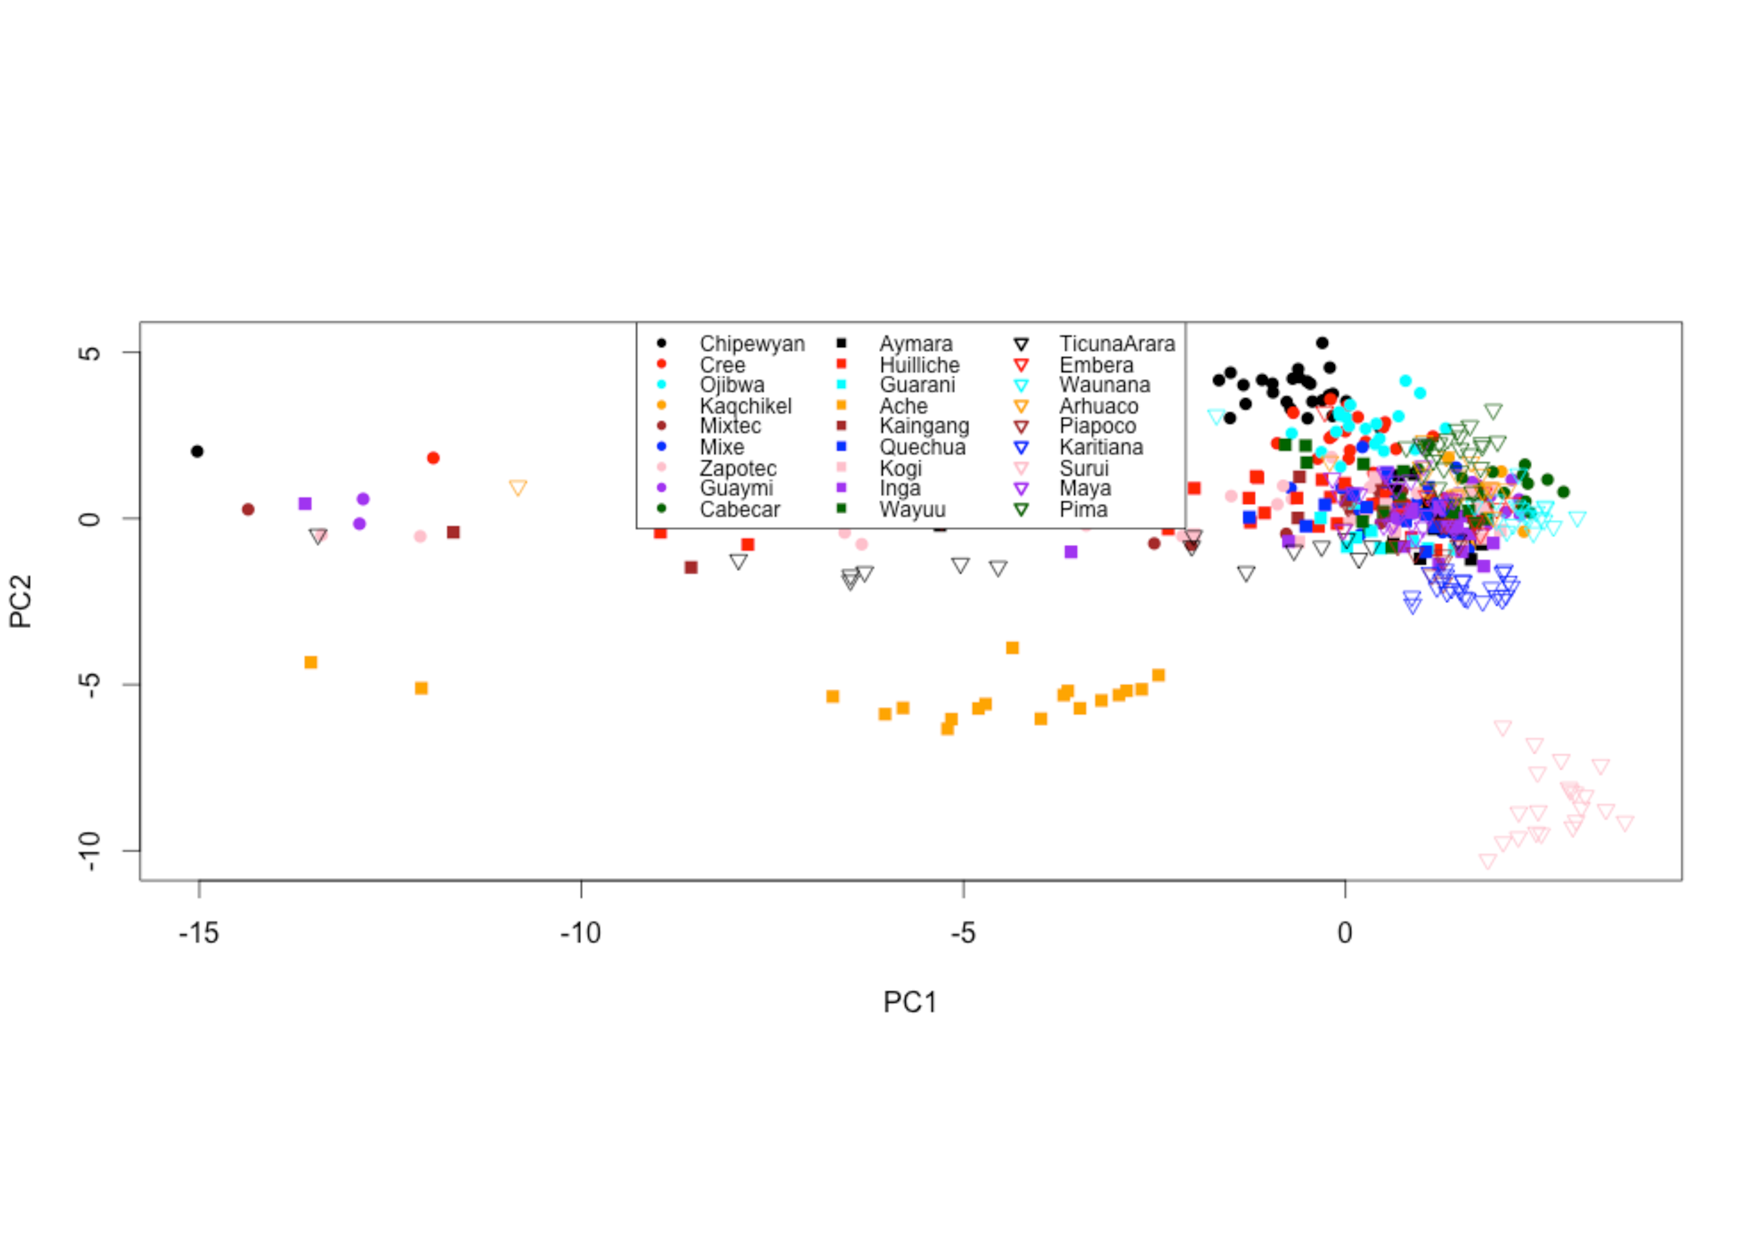
\includegraphics[scale=0.5]{Plot3b.pdf}
\caption{Les populations projetées sur les 2 premières PC}
\end{center}
\end{figure}

Avec les 2 premiers axes de l'ACP, les individus qui sont facilement identifiables sont les Surui et les Aches.
\pagebreak
\begin{figure}[!h]
\begin{center}
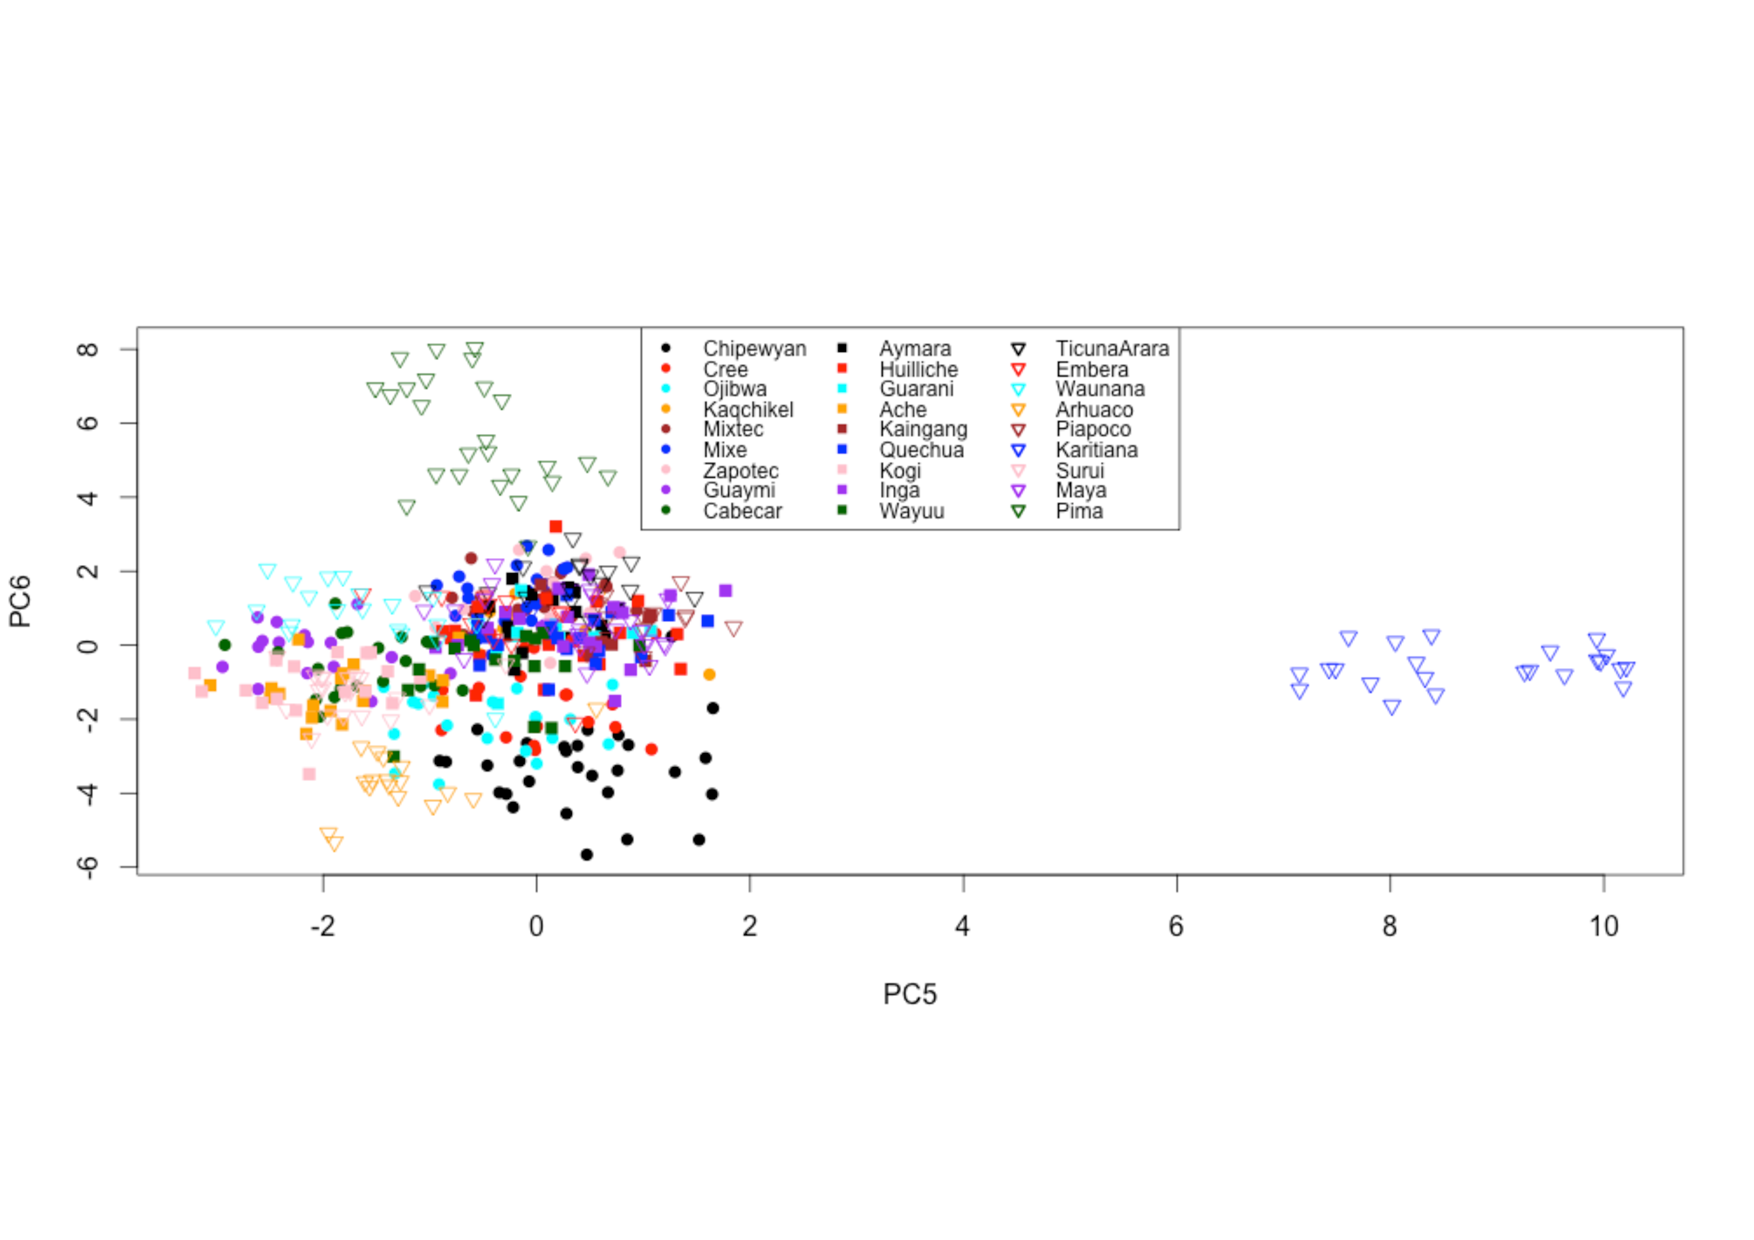
\includegraphics[scale=0.5]{Plot3b_bis.pdf}
\caption{Les populations projetées sur les PC 5 et 6}
\end{center}
\end{figure}

Avec les axes 5 et 6, ce sont les Karitiana et les Pima qui sont facilement identifiables. 

 \item[3.c)] 
 Le pourcentage cumulé de variance expliqué par les $2$ premières PC est de $3,57\%$. Elle est très faible donc l'ACP n'est pas réalisable : en retenant que les 2 premières PC, on ne peut pas bien expliquer le modèle. Pour avoir un pourcentage de variance correct ($70\%$) on va devoir garder 210 PC, ainsi on perdrait tout l'intérêt d'un ACP.

\end{enumerate}

\section{PCR Principal Companents Regression}

\begin{enumerate}
\setlength{\itemsep}{12pt}

\item[4.a)]
La régression de la latitude et de la longitude en utilisant comme prédicteurs les scores des 250 premiers axes de l'ACP nous donne que l'ACP1 n'influe pas sur la localisation même si elle maximise la variance des variables. Dans les deux régressions, la p-valeur de l'ACP1 est très grande (respectivement $0.44\%$ et $0.23\%$ pour la régression de la longitude et de la latitude) par rapport aux autres p-valeur des autres ACP. Donc il y a de forte chance que le coefficient de régression associé à ACP1 soit nul. 

\item[4.b)] 
Les coordonnées spatiales prédites pour chaque population sont localisées dans la même zone que les coordonnées réelles de chaque population. Cependant, on observe des erreurs : les coordonnées prédites peuvent être parfois très dispersée (comme les Huilliches). De plus, à cause de cette dispersion, on a beaucoup de mal à distinguer les populations qui sont situées très près les unes des autres (comme toutes celles d'Amériques centrales) : les points prédits se recoupent trop.

\begin{figure}[!h]
\begin{center}
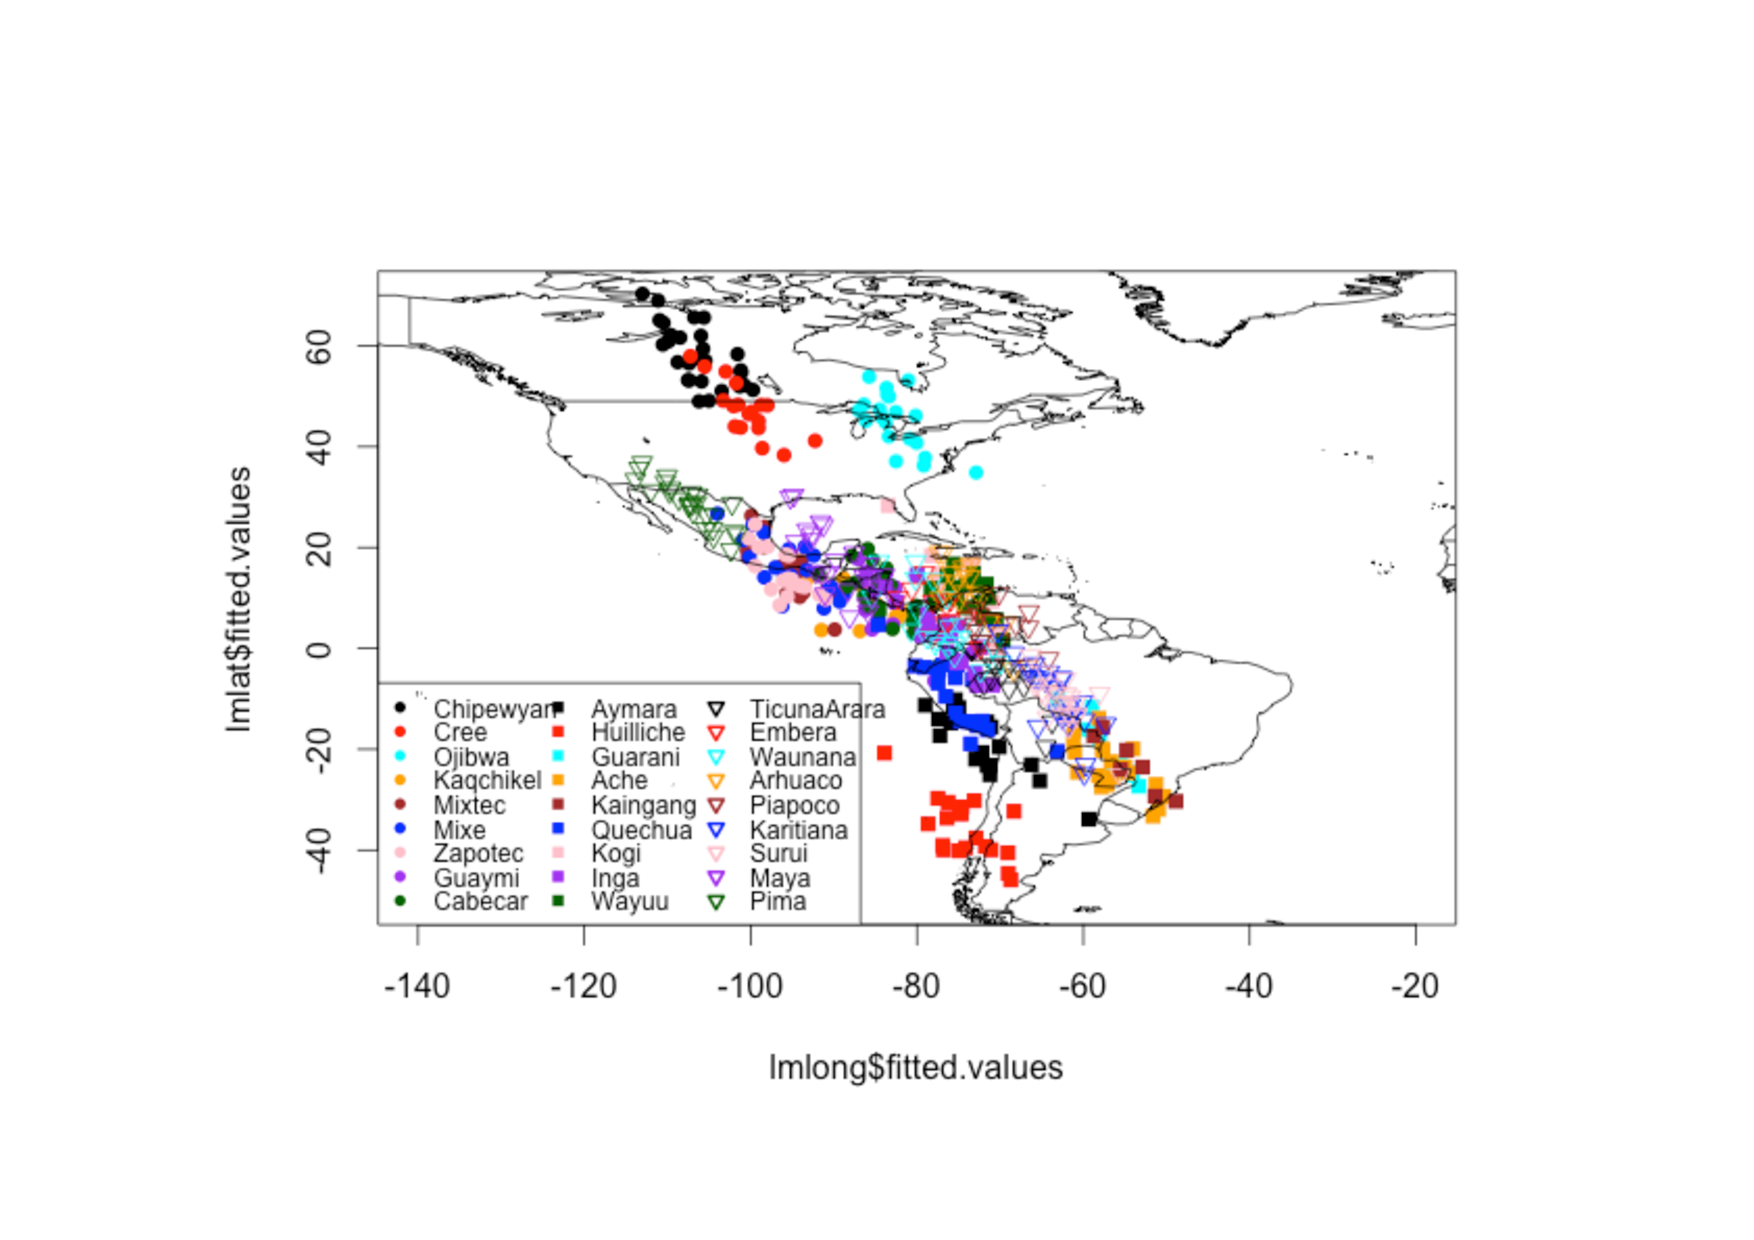
\includegraphics[scale=0.5]{Plot4b.pdf}
\caption{Coordonnées spatiales prédites pour chaque population}
\end{center}
\end{figure}

\item[4.c)]
Au final sur tous les écarts entre les valeurs prédites et valeurs réelles mesurés avec la distance du grand cercle on obtient 641km. Cette valeur a été obtenue en prenant la moyenne des écarts pour chaque population. C'est une valeur à relativiser. A l'échelle de l'Amérique ce n'est pas très grand et ce n'est pas si mal. Pour certaines populations cela se voit d'ailleurs, mais dès que les populations sont plus proche que cette distance on peine à les distinguer et donc notre modèle prédictif n'est pas très concluant pour ces populations.

\end{enumerate}

\end{document}

% TODO : parler du scrum master
